% ============================================================================
% FL-EHDS Paper v7 for FLICS 2026 — 8-page submission
% IEEE Conference Format (max 8 pages including references)
% March 2026
% ============================================================================

\documentclass[conference]{IEEEtran}
\IEEEoverridecommandlockouts

% ===== PACKAGES =====
\usepackage{cite}
\usepackage{amsmath,amssymb,amsfonts}
\usepackage{graphicx}
\usepackage{textcomp}
\usepackage{xcolor}
\usepackage{booktabs}
\usepackage{hyperref}
\usepackage{url}

% TikZ for vector figures
\usepackage{tikz}
\usetikzlibrary{shapes.geometric, arrows.meta, positioning, fit, backgrounds, calc}
\usepackage{pgfplots}
\pgfplotsset{compat=1.18}

% ===== DOCUMENT =====
\begin{document}

\title{FL-EHDS: A Privacy-Preserving Multimodal Federated Learning Framework for the European Health Data Space}

\author{
    \IEEEauthorblockN{Fabio Liberti}
    \IEEEauthorblockA{
        Department of Computer Science\\
        Universitas Mercatorum, Rome, Italy\\
        fabio.liberti@studenti.unimercatorum.it\\
        ORCID: 0000-0003-3019-5411
    }
}

\maketitle

% ============================================================================
% ABSTRACT
% ============================================================================
\begin{abstract}
The European Health Data Space (EHDS), established by Regulation (EU) 2025/327, mandates cross-border health data analytics while preserving citizen privacy. We present FL-EHDS, a three-layer compliance framework integrating EHDS governance (Health Data Access Bodies, data permits, Article~71 opt-out) with federated learning orchestration (17~algorithms including ICML/ICLR 2024--2025 advances, differential privacy, secure aggregation) and data holder components (FHIR~R4 preprocessing). Multimodal validation across 5,713+ experiments on tabular clinical, ECG, and medical imaging datasets demonstrates that \textit{personalization architecture---not aggregation algorithm---is the critical deployment decision}: only methods maintaining separate local models (Ditto, HPFL) differentiate from FedAvg on compact clinical models, producing up to 26.8pp accuracy gains---an advantage confirmed as hyperparameter-insensitive ($\leq$1.44pp across $100\times$ $\lambda$ variation), model-size invariant (2.9K--701K parameters), and persistent under compound EHDS stress ($+$9.6pp mean, 81\% of conditions). Privacy at $\varepsilon{=}10$ costs $<$2pp; cross-border heterogeneous per-client privacy budgets are viable ($-$0.9pp); full EHDS compliance (simultaneous data minimization, opt-out, and DP at $\varepsilon{=}10$) costs Ditto only $-$0.7pp ($p{<}0.001$). On imaging (ResNet-18), personalization is method-dependent: Ditto excels ($+$25.5pp Skin Cancer) while HPFL fails ($-$18.2pp Chest X-ray). A novel Diagnostic Equity Index reveals that accuracy masks severe per-class disparities correctable only by personalized algorithms. The open-source implementation provides deployment guidance for the 2029 secondary use deadline.
\end{abstract}

\begin{IEEEkeywords}
Federated Learning, European Health Data Space, Privacy-Preserving Technologies, Multimodal Health Analytics, GDPR, Health Data Governance, Cross-Border Analytics
\end{IEEEkeywords}

% ============================================================================
% 1. INTRODUCTION
% ============================================================================
\section{Introduction}
\label{sec:introduction}

The European Health Data Space (EHDS), established by Regulation (EU) 2025/327, creates a dual framework for cross-border health data governance: primary use through MyHealth@EU for patient care, and secondary use through HealthData@EU for research and policy-making~\cite{eu2025ehds}. Health Data Access Bodies (HDABs) in each Member State authorize secondary use through data permits; Article~53 enumerates permitted purposes; Article~71 introduces citizen opt-out mechanisms~\cite{staunton2024ethical}. The implementation timeline extends to 2031, with delegated acts expected by March 2027 and secondary use provisions applicable from March 2029.

Federated Learning (FL) is the key enabling technology for EHDS secondary use---the model travels to distributed data rather than centralizing sensitive records~\cite{mcmahan2017communication, kairouz2021advances}. Yet Fr\"ohlich et al.~\cite{frohlich2025reality} report that only 23\% of FL implementations achieve sustained production deployment, with hardware heterogeneity (78\%) and non-IID data (67\%) as dominant barriers. Beyond technical constraints, legal uncertainties regarding gradient data status under GDPR remain unresolved~\cite{quinn2024gdpr}, and privacy-enhancing technologies cannot substitute for robust governance frameworks~\cite{vandrumpt2025pets}.

Prior FL frameworks~\cite{rieke2020future, beutel2023flower, nvflare2023} focus on technical architectures without addressing regulatory compliance. Legal analyses~\cite{quinn2024gdpr, staunton2024ethical} examine GDPR constraints but abstract from implementation. No existing framework jointly addresses systematic barrier evidence, technical implementation with state-of-the-art algorithms, and EHDS governance operationalization---a gap confirmed by recent assessments~\cite{chaverodiez2026fair, teo2024systematic}.

This paper bridges the technology-governance divide through four contributions:
\begin{enumerate}
    \item \textbf{Barrier Taxonomy}: Evidence synthesis of 47 documents (PRISMA, GRADE-CERQual), identifying legal uncertainties as the critical adoption blocker.
    \item \textbf{FL-EHDS Framework}: A three-layer reference architecture mapping barriers to governance-aware mitigation strategies.
    \item \textbf{Reference Implementation}: Open-source codebase ($\sim$40K lines) with 17 FL algorithms, EHDS governance modules, and reproducible benchmarks.\footnote{\url{https://github.com/FabioLiberti/FL-EHDS-FLICS2026}}
    \item \textbf{Experimental Validation}: 5,713+ experiments demonstrating that personalization architecture---not aggregation strategy---is the critical EHDS deployment decision, with privacy at $\varepsilon{=}10$ essentially free and Article~71 opt-out fully compatible.
\end{enumerate}

% ============================================================================
% 2. BACKGROUND AND RELATED WORK
% ============================================================================
\section{Background and Related Work}
\label{sec:background}

\subsection{EHDS and Federated Learning}

The EHDS establishes HDABs to authorize secondary use through standardized data permits, with Secure Processing Environments (SPEs) providing controlled analytics~\cite{svingel2025hdab}. Implementation readiness varies significantly: Nordic countries hold 2--3 year advantages in HDAB capacity-building~\cite{tehdas2024ready}, while data access timelines range from 3~weeks (Finland) to over 12~months (France)~\cite{forster2025journeys}. Only 5.2\% of FL healthcare studies achieve real-life application~\cite{teo2024systematic}, with notable exceptions such as the EXAM COVID-19 study~\cite{dayan2021federated}.

FL inverts the traditional ML paradigm: local training produces gradients that are aggregated centrally~\cite{mcmahan2017communication}. Known challenges include non-IID distributions~\cite{li2020federated}, communication costs~\cite{bonawitz2019scale}, and privacy attacks~\cite{zhu2019deep, shokri2017membership}. Recent advances target healthcare heterogeneity: FedLESAM~\cite{qu2024fedlesam} (ICML 2024) provides globally-guided sharpness-aware optimization, while HPFL~\cite{chen2025hpfl} (ICLR 2025) decouples backbone from classifier for per-institution specialization.

\subsection{Related Frameworks}

Existing FL frameworks---Flower~\cite{beutel2023flower}, NVIDIA FLARE~\cite{nvflare2023}, and TensorFlow Federated~\cite{tff2019}---provide robust distributed training but lack EHDS-specific governance. A FAIR-based assessment of 17 FL frameworks~\cite{chaverodiez2026fair} confirms that none implements HDAB integration, data permit lifecycle, or opt-out enforcement. Table~\ref{tab:framework_comparison} provides a detailed comparison.

\begin{table}[htbp]
\centering
\caption{Framework Comparison: FL-EHDS vs Existing FL Frameworks}
\label{tab:framework_comparison}
\resizebox{\columnwidth}{!}{%
\begin{tabular}{lcccc}
\toprule
\textbf{Dimension} & \textbf{FL-EHDS} & \textbf{Flower v1.26} & \textbf{FLARE v2.7} & \textbf{TFF v0.88} \\
\midrule
FL Algorithms & 17 built-in & 12+ strategies & 5 built-in & 3 built-in \\
Byzantine Resilience & 6 methods & 4 methods & --- & --- \\
Differential Privacy & Central+Local & Central+Local & Built-in & Adaptive clip. \\
Secure Aggregation & Pairwise+HE & SecAgg+ & Built-in+HE & Mask-based \\
\midrule
EHDS Governance & \textbf{Full}$^\ddagger$ & None & None & None \\
HDAB Integration & \checkmark$^\ddagger$ & --- & --- & --- \\
Data Permits (Art.~53) & \checkmark$^\ddagger$ & --- & --- & --- \\
Opt-out (Art.~71) & \checkmark$^\ddagger$ & --- & --- & --- \\
\midrule
Healthcare Stds. & FHIR R4 & MONAI & MONAI & --- \\
Backend & PyTorch & Agnostic & Agnostic & TF only \\
\bottomrule
\end{tabular}%
}

\vspace{1mm}
\footnotesize{$^\ddagger$Reference implementation with simulation backend; production deployment requires binding to actual HDAB services (expected 2027--2029). See Supplementary Material, Table~S-ReadinessAssessment for readiness assessment.}
\end{table}

\subsection{Evidence Synthesis}

Following PRISMA 2020 guidelines, 847 records were screened; 47 met inclusion criteria (2022--2026, FL/EHDS focus). Table~\ref{tab:barriers} summarizes the five dominant barriers.

\begin{table}[htbp]
\caption{FL Implementation Barriers for EHDS}
\label{tab:barriers}
\centering
\small
\begin{tabular}{p{2.0cm}cp{2.0cm}p{1.8cm}}
\toprule
\textbf{Barrier} & \textbf{Prev.} & \textbf{Evidence} & \textbf{Mitigation} \\
\midrule
Hardware heterog. & 78\% & Fr\"ohlich 2025 & Adaptive engine \\
Non-IID data & 67\% & Multiple & FedProx, Ditto \\
Production gap & 23\% & Fr\"ohlich 2025 & Ref.\ implementation \\
FHIR compliance & 34\% & Hussein 2025 & Preprocessing \\
Communication cost & High & Bonawitz 2019 & Compression \\
\bottomrule
\end{tabular}
\end{table}

% ============================================================================
% 3. FL-EHDS FRAMEWORK
% ============================================================================
\section{FL-EHDS Framework}
\label{sec:framework}

Based on the identified barriers, we present FL-EHDS, a three-layer compliance framework for EHDS cross-border health analytics. Figure~\ref{fig:architecture} illustrates the architecture.

\begin{figure*}[t]
\centering
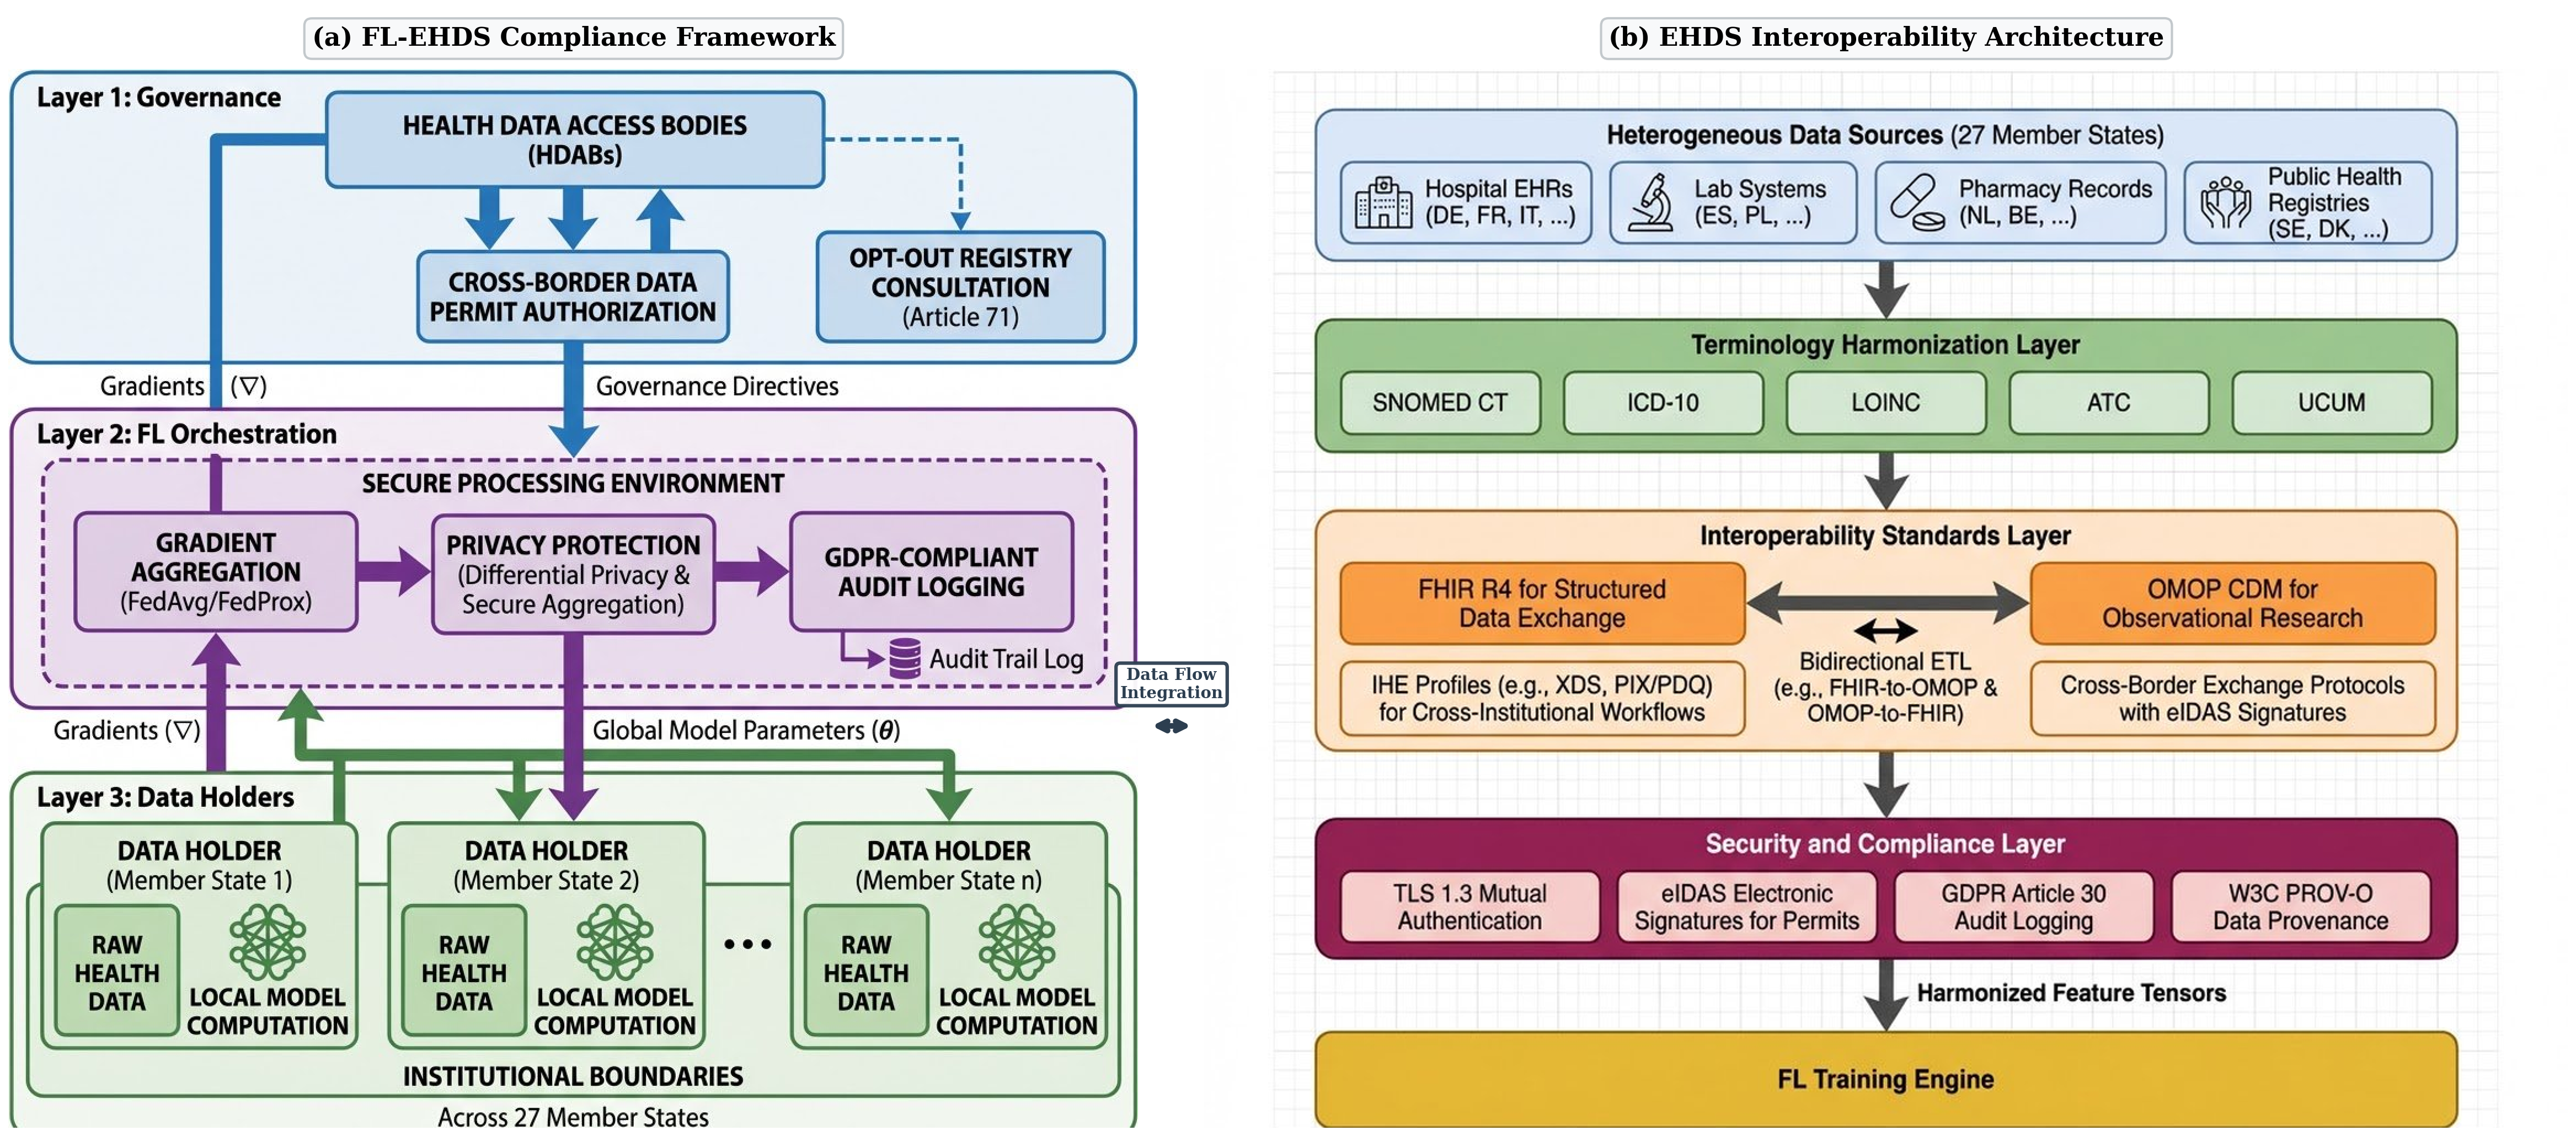
\includegraphics[width=\textwidth]{figures/fig1_composite_final}
\caption{FL-EHDS composite architecture.
(a)~Three-layer compliance framework: Layer~1 (Governance) manages
HDAB integration, data permit authorization, and Article~71 opt-out
registries; Layer~2 (FL Orchestration) operates within the Secure
Processing Environment with gradient aggregation, differential privacy,
and GDPR-compliant audit logging; Layer~3 (Data Holders) implements
local model computation with raw health data never leaving institutional
boundaries. (b)~EHDS interoperability pipeline: heterogeneous sources
across 27 Member States flow through terminology harmonization,
interoperability standards (FHIR~R4, OMOP~CDM, IHE profiles), and
security/compliance layers before reaching the FL training engine.}
\label{fig:architecture}
\end{figure*}

\textbf{Layer 1 -- Governance}: Standardized APIs for automated data permit verification before FL training initiation, designed to bind to production HDAB endpoints (expected 2027--2029). The governance layer manages the complete data permit lifecycle: per-round validation ensures that expired or revoked permits trigger immediate training termination; post-training, model artifacts are retained or deleted according to permit conditions. Multi-HDAB synchronization protocols coordinate cross-border studies under Article~41's single-application principle. National opt-out registries are consulted before each training epoch, ensuring Article~71 compliance at record-level granularity. Audit trails satisfy GDPR Article~30 requirements.

Algorithm~1 presents the core FL-EHDS training procedure with governance checkpoints.

\begin{figure}[htbp]
\centering
\fbox{\parbox{0.92\columnwidth}{
\small
\textbf{Algorithm 1: FL-EHDS FedAvg Training}\\[2pt]
\textbf{Input:} Hospitals $\mathcal{H} = \{h_1, \ldots, h_K\}$, permit $P$, rounds $T$\\
\textbf{Output:} Global model $\theta^{(T)}$\\[3pt]
\textbf{Server executes:}\\
\hspace*{4mm}Initialize $\theta^{(0)}$\\
\hspace*{4mm}\textit{// Cross-border coordination (Art.~41/46)}\\
\hspace*{4mm}\textbf{if} MultiCountry($P$) \textbf{then} SyncHDABs($P$.countries)\\
\hspace*{4mm}\textbf{for} round $t = 1$ to $T$ \textbf{do}\\
\hspace*{8mm}\textit{// Governance check (Layer 1)}\\
\hspace*{8mm}\textbf{if} not ValidatePermit($P$, $t$) \textbf{then abort}\\
\hspace*{8mm}$\mathcal{H}_t \leftarrow$ SelectParticipants($\mathcal{H}$)\\
\hspace*{8mm}\textbf{for each} $h \in \mathcal{H}_t$ \textbf{in parallel do}\\
\hspace*{12mm}$\Delta_h^{(t)}, n_h \leftarrow$ LocalTrain($h$, $\theta^{(t-1)}$)\\
\hspace*{8mm}\textit{// Aggregation with privacy (Layer 2)}\\
\hspace*{8mm}$\theta^{(t)} \leftarrow \theta^{(t-1)} + \frac{1}{\sum n_h} \sum_{h} n_h \cdot \Delta_h^{(t)}$\\
\hspace*{8mm}LogCompliance($t$, $\mathcal{H}_t$)\\[3pt]
\textbf{LocalTrain}($h$, $\theta$):\\
\hspace*{4mm}$\mathcal{D}_h \leftarrow$ FilterOptedOut($\mathcal{D}_h$, Registry) \textit{// Art.~71}\\
\hspace*{4mm}$\theta_h \leftarrow \theta$; train $E$ epochs on $\mathcal{D}_h$\\
\hspace*{4mm}$\Delta_h \leftarrow$ ClipGradient($\theta_h - \theta$, $C$) \textit{// DP bound}\\
\hspace*{4mm}\textbf{return} $\Delta_h$, $|\mathcal{D}_h|$
}}
\end{figure}

\textbf{Layer 2 -- FL Orchestration}: The framework implements 17 aggregation algorithms spanning six categories---from foundational methods (FedAvg~\cite{mcmahan2017communication}, FedProx~\cite{li2020federated}) through variance reduction (SCAFFOLD~\cite{karimireddy2020scaffold}), adaptive optimization~\cite{reddi2021adaptive}, and personalization (Ditto~\cite{li2021ditto}) to FedLESAM~\cite{qu2024fedlesam} (ICML 2024) and HPFL~\cite{chen2025hpfl} (ICLR 2025). The complete algorithm catalogue is provided in Supplementary Material, Table~S-AlgoCatalogue. Differential privacy uses DP-SGD~\cite{abadi2016deep} with R\'enyi composition~\cite{dwork2014dp, mironov2017renyi, wei2020federated}; secure aggregation with ECDH key exchange mitigates gradient inversion~\cite{zhu2019deep}; six Byzantine resilience methods defend against malicious clients. The threat model, covering honest-but-curious server, malicious clients, and external attackers, is detailed in Supplementary Material, Section~S-Threat.

\textbf{Layer 3 -- Data Holders}: Resource-aware training engines dynamically adjust batch sizes and model complexity for hardware heterogeneity (78\% barrier prevalence). FHIR~R4 preprocessing pipelines bridge format gaps across heterogeneous EHR systems~\cite{hussein2025interop}. End-to-end encrypted gradient transmission ensures no raw data leaves institutional boundaries.

\textbf{EHDS Compliance Mapping}: Table~\ref{tab:compliance} maps framework components to regulatory requirements with explicit enforcement mechanisms. FL-EHDS implements governance-ready abstractions with pluggable HDAB connectors: the current release provides simulation backends for reproducible experimentation; production binding requires connector configuration only, not architectural changes---a design validated by the modular API boundary (Supplementary Material, Table~S-ReadinessAssessment).

\begin{table}[htbp]
\caption{EHDS Compliance Mapping}
\label{tab:compliance}
\centering
\small
\resizebox{\columnwidth}{!}{%
\begin{tabular}{lp{1.6cm}p{1.6cm}p{3.0cm}}
\toprule
\textbf{Article} & \textbf{Requirement} & \textbf{Component} & \textbf{Enforcement Mechanism} \\
\midrule
Art. 33 & Secondary use auth. & HDAB API + Permit valid. & Per-round permit check; training aborts on expiry/revocation \\
Art. 37 & Data quality labels & Quality gate & Pre-training validation of completeness and label consistency \\
Art. 41 & Single application (multi-country) & Multi-HDAB coord. & Unified permit request routed to lead HDAB with parallel sync \\
Art. 46 & Cross-border proc. & Cross-border orch. & Per-client heterogeneous $\varepsilon$ with HDAB-specified budgets \\
Art. 49 & SPE security req. & SPE boundary enf. & Encrypted aggregation; no raw data egress; audit logging \\
Art. 50 & Secure Proc.\ Env. & Aggregation in SPE & Gradient-only exchange; model never exposes individual records \\
Art. 53 & Permitted purposes & Purpose limitation & Permit-bound purpose codes validated before each training job \\
Art. 55 & Data holder oblig. & Layer~3 data engine & FHIR~R4 format compliance; response within regulatory timelines \\
Art. 71 & Opt-out mechanism & Registry filtering & Record-level exclusion before each epoch; dynamic mid-training withdrawal \\
\bottomrule
\end{tabular}%
}
\end{table}

The per-round audit trail produced by LogCompliance() (Algorithm~1) directly supports Data Protection Impact Assessment (DPIA) obligations under GDPR Article~35, documenting processing scope, participant selection, and privacy parameters for each training round---reducing DPIA burden compared to centralized alternatives where raw data leaves institutional boundaries.

% ============================================================================
% 4. EXPERIMENTAL EVALUATION
% ============================================================================
\section{Experimental Evaluation}
\label{sec:experiments}

\subsection{Setup}

We evaluate FL-EHDS on real clinical datasets simulating cross-border healthcare analytics. All results are reproducible via the benchmark suite.

\textbf{Datasets}: Table~\ref{tab:dataset_coverage} summarizes 8 datasets spanning tabular EHR and medical imaging across three scale regimes (569--101K samples). PTB-XL ECG~\cite{wagner2020ptbxl}---European-origin, 21,799 records from 52 German recording sites with natural hospital partitioning---is uniquely representative of real EHDS cross-institutional heterogeneity. \textbf{Models}: HealthcareMLP (2-layer, 64/32 hidden, $\sim$10K parameters) for tabular; ResNet-18~\cite{he2016deep} ($\sim$11.2M parameters) for imaging. \textbf{Configuration}: Per-dataset optimized hyperparameters (Supplementary Material, Table~S-DatasetConfig); mean $\pm$ std over 3+ seeds; Adam optimizer; early stopping with patience=6.

\begin{table}[htbp]
\centering
\caption{Evaluated Dataset Coverage}
\label{tab:dataset_coverage}
\resizebox{\columnwidth}{!}{%
\begin{tabular}{lcccl}
\toprule
\textbf{Dataset} & \textbf{Samples} & \textbf{Feat.} & \textbf{Cls.} & \textbf{FL Partition} \\
\midrule
\multicolumn{5}{l}{\textit{Tabular Clinical (MLP, $\sim$10K params)}} \\
Heart Disease UCI & 920 & 13 & 2 & Natural (4 hosp.) \\
Breast Cancer Wisc. & 569 & 30 & 2 & Dirichlet \\
PTB-XL ECG$^\dagger$ & 21,799 & 9 & 5 & Natural (52 EU sites) \\
Diabetes 130-US & 101,766 & 22 & 2 & Dirichlet \\
Cardiovascular & 70,000 & 11 & 2 & Dirichlet \\
\midrule
\multicolumn{5}{l}{\textit{Medical Imaging (ResNet-18, $\sim$11.2M params)}} \\
Chest X-ray & 5,856 & --- & 2 & Dirichlet \\
Brain Tumor MRI & 7,023 & --- & 4 & Dirichlet \\
Skin Cancer & 3,297 & --- & 2 & Dirichlet \\
\bottomrule
\end{tabular}%
}

\vspace{1mm}
\footnotesize{$^\dagger$European-origin (PTB, Berlin), SCP-ECG standard, 5-class cardiac diagnosis. 52 recording sites grouped into $K$ geographic clusters (default $K{=}5$).}
\end{table}

\subsection{Algorithm Comparison}

Table~\ref{tab:tabular_main} presents the primary evaluation: 7 algorithms on PTB-XL, Cardiovascular, and Breast Cancer. Together with supplementary validation on Heart Disease, Diabetes, imaging, extended experiments (server-side optimizers, CDC Diabetes 253K, 10-seed robustness, vertical FL), and thesis robustness validation (below), the evaluation comprises 5,713+ experiments (Supplementary Material, Table~S-ExperimentMap).

\begin{table*}[htbp]
\centering
\caption{FL Algorithm Comparison on Real Clinical Datasets (7 Algorithms $\times$ 3 Datasets). Best accuracy per dataset in \textbf{bold}. Mean $\pm$ std over 5 seeds. PX = PTB-XL ECG (5 clients, 5-class, site-based), CV = Cardiovascular (5 clients, binary, $\alpha$=0.5), BC = Breast Cancer (3 clients, binary, $\alpha$=0.5).}
\label{tab:tabular_main}
\resizebox{\textwidth}{!}{%
\begin{tabular}{lccccccccc}
\toprule
\textbf{Algorithm} & \multicolumn{3}{c}{\textbf{PTB-XL ECG (21,799 records, 52 EU sites)}} & \multicolumn{3}{c}{\textbf{Cardiovascular (70K patients)}} & \multicolumn{3}{c}{\textbf{Breast Cancer (569 samples)}} \\
\cmidrule(lr){2-4}\cmidrule(lr){5-7}\cmidrule(lr){8-10}
 & Acc (\%) & F1 (\%) & Jain & Acc (\%) & F1 (\%) & Jain & Acc (\%) & F1 (\%) & Jain \\
\midrule
FedAvg & 91.9$\pm$0.5 & 88.3 & 0.999 & 71.1$\pm$1.8 & 68.8 & 0.981 & 52.3$\pm$17.9 & 32.0 & 0.608 \\
FedProx & 91.6$\pm$0.7 & 87.4 & 0.999 & 71.5$\pm$1.2 & 69.6 & 0.986 & 52.3$\pm$17.9 & 32.0 & 0.608 \\
\textbf{Ditto} & 91.8$\pm$0.3 & 88.8 & 0.999 & \textbf{82.5$\pm$4.7} & 82.3 & 0.980 & \textbf{79.1$\pm$12.5} & 64.5 & 0.606 \\
FedLC & 91.9$\pm$0.5 & 88.2 & 0.999 & 71.1$\pm$1.6 & 68.8 & 0.982 & 52.1$\pm$18.1 & 32.6 & 0.606 \\
FedExP & 92.0$\pm$0.2 & 89.2 & 0.999 & 71.1$\pm$1.8 & 68.8 & 0.981 & 52.3$\pm$17.9 & 32.0 & 0.608 \\
FedLESAM & 91.9$\pm$0.5 & 88.3 & 0.999 & 71.1$\pm$1.8 & 68.8 & 0.981 & 52.3$\pm$17.9 & 32.0 & 0.608 \\
\textbf{HPFL} & \textbf{92.5$\pm$0.3} & \textbf{89.7} & 0.999 & 82.3$\pm$4.5 & 82.0 & 0.984 & 74.1$\pm$20.9 & 62.1 & 0.867 \\
\bottomrule
\end{tabular}%
}
\par{\footnotesize F1 = positive-class binary (CV, BC) / macro-averaged (PTB-XL, 5-class); BC std from single-class collapse (see text).}
\end{table*}

\textbf{Key findings}:

\begin{enumerate}
    \item \textbf{Personalization architecture is the critical design choice}: On compact tabular models ($\sim$10K parameters), five of seven algorithms (FedLESAM, FedExP, FedLC, FedProx, FedAvg) converge to statistically identical solutions---confirmed by server-side optimizer experiments where FedAdam, FedYogi, and FedAdagrad also produce identical results ($p{>}0.9$, Kruskal--Wallis; Supplementary Material, Table~S-ServerOpt). Only methods maintaining separate local models (Ditto, HPFL) differentiate. This simplifies EHDS deployment to a single architectural choice: personalized vs.\ global.

    \item \textbf{Personalization dominates across scales}: Ditto and HPFL consistently outperform baselines---11.2pp on Heart Disease, 11.4pp on Cardiovascular, 26.8pp on Breast Cancer. Extended 10-seed validation confirms $p < 0.001$ (pooled Wilcoxon). HPFL uniquely improves fairness (Jain 0.867 vs.\ 0.608 on Breast Cancer).

    \item \textbf{PTB-XL validates European FL}: The European-origin PTB-XL with natural 52-site partitioning achieves 92.5\% accuracy (HPFL) with near-perfect fairness (Jain 0.999)---demonstrating FL viability for real European multi-center clinical data.

    \item \textbf{Diagnostic equity is algorithm-dependent}: We introduce the Diagnostic Equity Index (DEI~$= \min_c R_c \cdot (1 - \text{CV}(\mathbf{R}))$), revealing that FedAvg achieves 52.8\% mean accuracy (median 59.4\%) but DEI as low as 0.092 on Breast Cancer---a bimodal distribution where 5/10 seeds suffer single-class collapse (mean 41.5\%) while 5/10 reach 64.2\%, underscoring that aggregate accuracy masks catastrophic diagnostic failures detectable only through DEI. HPFL reaches DEI~$=$~0.740 ($8\times$). On Brain Tumor, Ditto DEI~$=$~0.435 vs.\ FedAvg 0.063 ($6.9\times$). EHDS data permits should specify minimum DEI thresholds (Supplementary Material, Section~S-DEI).

    \item \textbf{Imaging personalization is method-dependent}: Table~\ref{tab:imaging_main} extends the evaluation to medical imaging with ResNet-18 (11.2M parameters). The personalization effect reverses: Ditto achieves $+$23.5pp on Brain Tumor ($p{=}0.015$) and $+$25.5pp on Skin Cancer, while HPFL is counterproductive on all imaging tasks ($-$3.8pp to $-$18.2pp). The distinction is architectural: Ditto preserves full CNN capacity via complete local copies, while HPFL's split-head cannot learn shared representations under non-IID imaging distributions. Notably, on Chest X-ray (binary, 5.8K samples), global aggregation suffices and personalization degrades performance---demonstrating that the optimal architecture depends on both modality and task complexity (Supplementary Material, Section~S-Imaging).
\end{enumerate}

\begin{table}[htbp]
\centering
\caption{Medical imaging evaluation (ResNet-18, 11.2M params). 5 clients, Dirichlet $\alpha{=}0.5$, 20 rounds, early stopping. Mean over 3 seeds. Best per dataset in \textbf{bold}.}
\label{tab:imaging_main}
\small
\begin{tabular}{lccccc}
\toprule
\textbf{Dataset} & \textbf{FedAvg} & \textbf{FedLESAM} & \textbf{Ditto} & \textbf{HPFL} & \textbf{DEI$^\S$} \\
\midrule
Chest X-ray & 87.3\% & \textbf{87.8}\%$^\dagger$ & 80.0\% & 69.1\% & .528/.652 \\
Brain Tumor & 53.8\% & 53.8\%$^\dagger$ & \textbf{77.3}\% & 50.0\% & .063/.435 \\
Skin Cancer & 65.0\% & 65.0\%$^\dagger$ & \textbf{90.5}\% & 60.9\% & --- \\
\bottomrule
\end{tabular}

\vspace{1mm}
\footnotesize{$^\dagger$FedLESAM $\equiv$ FedAvg: per-seed accuracies identical on Brain Tumor and Skin Cancer, $<$1.2pp difference on Chest X-ray---confirming that the global algorithm convergence extends to imaging. 4 additional global algorithms confirm this pattern (Supplementary Material). $^\S$DEI column: FedAvg/best-personalized. On Brain Tumor, Ditto DEI (0.435) is $6.9\times$ FedAvg (0.063); on Chest X-ray, HPFL DEI (0.652) exceeds FedAvg (0.528) despite lower accuracy (Supplementary Material, Table~S-DEI).}
\end{table}

\subsection{Convergence and Paradigm Comparison}

Figure~\ref{fig:convergence} shows representative training convergence on Heart Disease UCI (4 hospitals, natural non-IID); Ditto achieves an 11.2pp advantage over FedAvg from personalized local models, while SCAFFOLD exhibits high variance due to control variate instability. Table~\ref{tab:fl_vs_central} compares five approaches across 10 seeds: Local-Only achieves high accuracy (78.6\%) but poor F1 (0.582) and undefined AUC, masking class-imbalance issues that only collaborative learning resolves. FL-Ditto approaches centralized performance (3.6pp gap) while preserving full data sovereignty.

\begin{figure}[htbp]
\centering
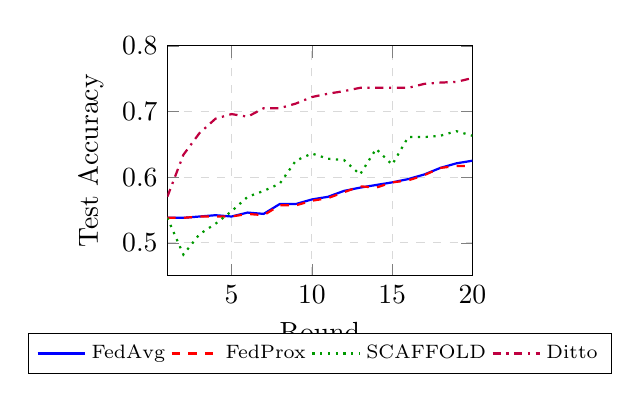
\begin{tikzpicture}
\begin{axis}[
    width=0.45\textwidth,
    height=4.5cm,
    xlabel={Round},
    ylabel={Test Accuracy},
    legend style={at={(0.5,-0.25)}, anchor=north, font=\scriptsize, legend columns=4},
    grid=major,
    grid style={dashed, gray!30},
    xmin=1, xmax=20,
    ymin=0.45, ymax=0.80,
]
\addplot[blue, thick] coordinates {(1,0.538) (2,0.538) (3,0.540) (4,0.542) (5,0.540) (6,0.546) (7,0.544) (8,0.559) (9,0.559) (10,0.566) (11,0.570) (12,0.579) (13,0.584) (14,0.588) (15,0.592) (16,0.597) (17,0.604) (18,0.614) (19,0.621) (20,0.625)};
\addplot[red, thick, dashed] coordinates {(1,0.538) (2,0.538) (3,0.540) (4,0.540) (5,0.540) (6,0.544) (7,0.542) (8,0.557) (9,0.557) (10,0.564) (11,0.568) (12,0.577) (13,0.586) (14,0.584) (15,0.592) (16,0.595) (17,0.603) (18,0.614) (19,0.617) (20,0.617)};
\addplot[green!60!black, thick, dotted] coordinates {(1,0.538) (2,0.482) (3,0.513) (4,0.529) (5,0.548) (6,0.570) (7,0.579) (8,0.590) (9,0.625) (10,0.636) (11,0.628) (12,0.626) (13,0.604) (14,0.643) (15,0.619) (16,0.661) (17,0.661) (18,0.663) (19,0.670) (20,0.663)};
\addplot[purple, thick, dashdotted] coordinates {(1,0.570) (2,0.634) (3,0.667) (4,0.689) (5,0.696) (6,0.692) (7,0.705) (8,0.705) (9,0.712) (10,0.722) (11,0.727) (12,0.731) (13,0.736) (14,0.736) (15,0.736) (16,0.736) (17,0.742) (18,0.744) (19,0.745) (20,0.751)};
\legend{FedAvg, FedProx, SCAFFOLD, Ditto}
\end{axis}
\end{tikzpicture}
\caption{Training convergence on Heart Disease UCI (4 hospitals, natural non-IID). Ditto converges faster and higher due to personalized local models.}
\label{fig:convergence}
\end{figure}

\begin{table}[htbp]
\centering
\caption{Learning Paradigm Comparison (Heart Disease UCI)}
\label{tab:fl_vs_central}
\small
\begin{tabular}{lcccc}
\toprule
\textbf{Approach} & \textbf{Acc.} & \textbf{F1} & \textbf{AUC} & \textbf{Gap} \\
\midrule
Centralized & $79.6 \pm 5.0$\% & $.789$ & $.873$ & --- \\
Local-Only & $78.6 \pm 2.9$\% & $.582$ & ---$^\dagger$ & 1.0pp \\
FL-Ditto & $76.0 \pm 2.3$\% & $.772$ & $.819$ & 3.6pp \\
FL-HPFL & $75.0 \pm 2.8$\% & $.756$ & $.810$ & 4.6pp \\
FL-FedAvg & $64.8 \pm 7.9$\% & $.753$ & $.846$ & 14.8pp \\
\bottomrule
\end{tabular}

\vspace{1mm}
\footnotesize{4 hospitals, natural non-IID. Mean $\pm$ std over 10 seeds. FL: 20 rounds $\times$ 3 local epochs. $^\dagger$Local-Only AUC undefined: single-class test partitions at some hospitals prevent ROC computation. Extended results in Supplementary Material, Table~S-HD-Diabetes.}
\end{table}

\subsection{Non-IID Impact and Compound Stress}

Figure~\ref{fig:noniid_impact} shows the impact of data heterogeneity on algorithm performance across all 17 FL-EHDS algorithms (Cardiovascular, No-DP, 5 seeds per condition, 210 experiments). As non-IID severity increases ($\alpha \to 0$), algorithm selection becomes critical. Of 17 algorithms, 10 cluster within 3pp of FedAvg at $\alpha{=}0.5$---including Per-FedAvg (MAML-based personalization), confirming that not all personalization strategies differentiate. Counter-intuitively, HPFL \textit{improves} under extreme heterogeneity ($\alpha{=}0.1$: $94.8 \pm 5.6$\% vs.\ $81.2 \pm 3.1$\% at $\alpha{=}1.0$), while FedAvg, Ditto, and 8 other algorithms remain indistinguishable. SCAFFOLD's control variates are unstable with few heterogeneous clients ($-$24pp at $\alpha{=}0.1$). This confirms that \textit{specific personalization architecture} (split-head), not aggregation strategy or generic personalization, determines robustness to heterogeneity.

\begin{figure}[htbp]
\centering
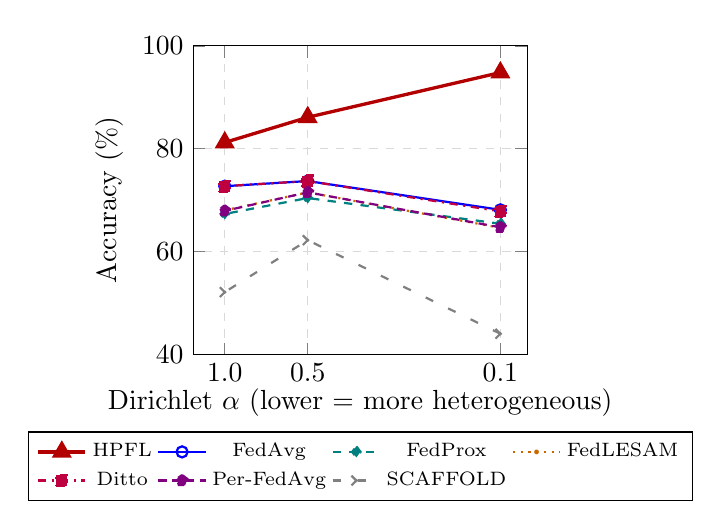
\begin{tikzpicture}
\begin{axis}[
    width=0.48\textwidth,
    height=5.5cm,
    xlabel={Dirichlet $\alpha$ (lower = more heterogeneous)},
    ylabel={Accuracy (\%)},
    legend style={at={(0.5,-0.25)}, anchor=north, font=\scriptsize, legend columns=4},
    grid=major,
    grid style={dashed, gray!30},
    xmode=log,
    xtick={0.1, 0.5, 1.0},
    xticklabels={0.1, 0.5, 1.0},
    xmin=0.08, xmax=1.3,
    ymin=40, ymax=100,
    every axis x label/.style={at={(0.5,-0.08)}, anchor=north},
    x dir=reverse,
]
% HPFL — the only outperformer (split-head personalization)
\addplot[red!70!black, very thick, mark=triangle*, mark size=3pt] coordinates {(0.1,94.8) (0.5,86.1) (1.0,81.2)};
% Global algorithms cluster (representative selection)
\addplot[blue, thick, mark=o, mark size=2pt] coordinates {(0.1,68.1) (0.5,73.7) (1.0,72.7)};
\addplot[teal, thick, dashed, mark=diamond*, mark size=2pt] coordinates {(0.1,65.4) (0.5,70.4) (1.0,67.3)};
\addplot[orange!80!black, thick, dotted, mark=star, mark size=2.5pt] coordinates {(0.1,64.6) (0.5,71.5) (1.0,68.0)};
% Personalized algorithms that do NOT differentiate
\addplot[purple, thick, dashdotted, mark=square*, mark size=2pt] coordinates {(0.1,67.8) (0.5,73.7) (1.0,72.7)};
\addplot[violet, thick, densely dashed, mark=pentagon*, mark size=2pt] coordinates {(0.1,64.7) (0.5,71.5) (1.0,67.9)};
% SCAFFOLD — non-IID specialist that fails
\addplot[gray, thick, loosely dashed, mark=x, mark size=2.5pt] coordinates {(0.1,44.0) (0.5,62.2) (1.0,52.1)};
\legend{HPFL, FedAvg, FedProx, FedLESAM, Ditto, Per-FedAvg, SCAFFOLD}
\end{axis}
\end{tikzpicture}
\caption{Accuracy vs.\ data heterogeneity on Cardiovascular (No-DP, mean over 4--5 seeds, 7 of 17 algorithms shown). All 17 algorithms were evaluated (210 additional experiments); 10 cluster within 3pp of FedAvg. Only HPFL's split-head architecture benefits from heterogeneity ($+$26.7pp over FedAvg at $\alpha{=}0.1$). SCAFFOLD's control variates are unstable with few heterogeneous clients. Complete results for all 17 algorithms in Supplementary Material (Table~S-NonIID-17algo).}
\label{fig:noniid_impact}
\end{figure}

The interaction between non-IID data and DP is \textit{sub-additive for HPFL} but \textit{super-additive for FedAvg/Ditto} (126 experiments, 4--5 seeds per condition). Under extreme heterogeneity ($\alpha{=}0.1$) with $\varepsilon{=}1$, HPFL retains $91.3 \pm 10.4$\% ($-$3.5pp from no-DP) while Ditto collapses to $51.3 \pm 5.8$\% ($-$16.5pp)---HPFL's personalized heads absorb heterogeneity, leaving less surface for DP noise. Under compound stress combining non-IID ($\alpha{=}0.1$), DP ($\varepsilon{=}10$), and partial participation (60\%) simultaneously (48 experiments), HPFL's worst-case accuracy (86.2\% on Cardiovascular) exceeds FedAvg's \textit{best}-case (72.6\%) by 13.6pp (Supplementary Material, Tables~S-NonIID-DP, S-CompoundStress). Real EHDS deployments face all three constraints simultaneously; only HPFL survives compound stress.

\textbf{Thesis robustness validation}: 516 additional experiments stress-test the personalization thesis (Supplementary Material, Section~S-ThesisRobustness). Ditto's $\lambda$ across $100\times$ range produces $\leq$1.44pp variation (75~exp.)---the advantage is not a tuning artifact. Personalization emerges at $\geq$25\% data fraction (225~exp.), with Ditto reaching $+$11.2pp over FedAvg at 25\% on Cardiovascular---enabling near-optimal EHDS analytics during phased rollout. Under compound stress (216~exp.\ covering IID/non-IID $\times$ DP $\times$ participation $\times$ opt-out), Ditto outperforms FedAvg in 81\% of conditions ($+$9.6pp mean); worst-case: 72.6\% vs.\ 52.4\% ($+$20.2pp).

\subsection{Privacy and EHDS Compliance}

Table~\ref{tab:dp_mini} summarizes the privacy-utility tradeoff on PTB-XL. At $\varepsilon{=}10$, all algorithms recover to within 1pp of no-DP baselines; at $\varepsilon{=}1$, only personalized methods retain $>$87\% accuracy while FedAvg collapses to 52.3\%. Across 180 DP experiments, privacy at $\varepsilon{=}10$ is essentially free ($<$2pp cost), satisfying EHDS Article~50 SPE requirements. On small datasets (Breast Cancer, 569 samples), DP acts as implicit regularization: FedAvg improves from 52.3\% to 78.7\% with $\varepsilon{=}5$ ($+$26.4pp). This regularization effect extends to population scale: on CDC Diabetes (253K samples), FedAvg improves from 70.1\% to 85.8\% at $\varepsilon{=}5$ (Supplementary Material, Section~S-CDC).

\begin{table}[htbp]
\centering
\caption{Privacy-utility on PTB-XL ECG: accuracy (\%) under central DP. Gaussian mechanism, $C{=}1.0$, $\delta{=}10^{-5}$. Mean over 5 seeds.}
\label{tab:dp_mini}
\small
\begin{tabular}{lcccc}
\toprule
\textbf{Algorithm} & $\boldsymbol{\varepsilon{=}1}$ & $\boldsymbol{\varepsilon{=}10}$ & $\boldsymbol{\varepsilon{=}50}$ & \textbf{No DP} \\
\midrule
FedAvg & 52.3 & \textbf{92.4} & 92.4 & 91.9 \\
Ditto & 89.2 & 91.6 & 91.9 & 91.8 \\
HPFL & 87.1 & 92.4 & \textbf{92.7} & 92.5 \\
\bottomrule
\end{tabular}
\end{table}

\textbf{Cross-border privacy heterogeneity}: Under the realistic scenario of 2 German clients ($\varepsilon{=}1$) federating with 3 Italian clients ($\varepsilon{=}10$) on PTB-XL, heterogeneous per-client local DP is viable: Ditto loses only $-$0.9pp vs.\ no-DP, and FedAvg with mixed budgets (89.3\%) \textit{outperforms} the strictest-wins rule (85.6\%, $+$3.8pp). HPFL collapses under local DP (54.4\% at $\varepsilon{=}1$) because per-client noise corrupts its shared backbone---requiring careful algorithm-privacy architecture co-design. \textit{No prior FL work we are aware of experimentally evaluates heterogeneous per-client DP budgets} (Supplementary Material, Table~S-CrossBorder).

\textbf{Article~71 compliance}: Static opt-out at 5--30\% rates (225 experiments) costs $<$1pp on adequately-sized datasets. Dynamic mid-training withdrawal of 1--2 clients (90 experiments) costs $<$1pp; Ditto and HPFL are shock-resistant (0.0pp immediate drop). \textit{Mid-training client withdrawal has not been systematically studied in prior FL work} (Supplementary Material, Tables~S-Optout, S-DynOptout).

\textbf{Compound EHDS governance validation}: 720 hypothesis-driven experiments validate the \textit{simultaneous} application of Article~44 data minimization, Article~71 opt-out, and Recital~57 differential privacy on Heart Disease (920 samples, 4~hospitals) and Cardiovascular (70K samples, 5~clients). Under full compliance (11$\to$4 features, 10\% opt-out, $\varepsilon{=}10$), Ditto loses only $-$0.7pp ($p{<}0.001$) and HPFL $-$1.7pp ($p{=}0.004$) on CV---confirming that full EHDS compliance is essentially free for personalized algorithms. Non-uniform opt-out patterns---including 50\% from a single hospital---produce no significant fairness degradation (Jain$\geq$0.96, all $p{>}0.73$). A novel \textit{governance resilience} metric ($R = \text{acc}_{\text{purpose}} / \text{acc}_{\text{sci.\ research}}$) reveals a critical gap: Ditto/HPFL retain 94.8\% accuracy under official statistics purpose (82\% feature reduction) vs.\ FedAvg 84.7\%. Cross-dataset validation confirms all Heart Disease paradoxes (governance improving accuracy) as small-sample regularization artifacts absent on CV (Supplementary Material, Section~S-GovernanceHypotheses).

\textbf{Membership inference resistance}: FedAvg and Ditto are inherently immune (attack AUC$\approx$0.50); HPFL is vulnerable (AUC~$=$~0.666) due to personalized heads. DP at $\varepsilon{=}1$ resolves this (AUC$\to$0.337)---revealing a \textit{privacy--personalization tension} that EHDS data permits should address. Gradient inversion attacks (DLG~\cite{zhu2019deep}) achieve successful reconstruction without DP on PTB-XL (cosine similarity 0.816), but $\varepsilon{=}10$ completely prevents reconstruction (100\% attack failure, cosine$\to$0.021; Supplementary Material, Table~S-MIA).

\textbf{Centralized--FL gap}: Centralized baselines on PTB-XL (92.6$\pm$0.4\%), Cardiovascular (73.5$\pm$0.3\%), and CDC Diabetes (86.5$\pm$0.1\%) confirm that the FL gap is $\leq$0.5pp on adequately-sized datasets---negligible compared to the algorithm selection effect (Supplementary Material, Table~S-CentralBaseline).

\textbf{Data efficiency}: All algorithms reach within 1\% of full-data performance with only 50\% of training data across all datasets, enabling near-optimal EHDS analytics during phased hospital participation in the 2025--2031 rollout (Supplementary Material, Table~S-DataEfficiency).

\textbf{Communication and scalability}: Tabular FL requires 0.04~MB/round (0.8~MB total for 20 rounds); imaging (ResNet-18) requires 44.7~MB/round, reducible by 95\% via Top-$k$ sparsification. Client scaling from 3 to 20 hospitals (135 experiments) shows graceful degradation ($-$4.8pp); HPFL is the most scalable under DP: 64.6\% at $K{=}20$ vs.\ FedAvg 55.4\% ($+$9.2pp). Top-$k$ and DP exhibit a synergy for HPFL: Top-1\% with $\varepsilon{=}1$ \textit{improves} accuracy to 85.6\% (vs.\ 75.5\% without sparsification), as sparsification regularizes against DP noise (Supplementary Material, Tables~S-CommCosts, S-Scalability, S-DP-TopK).

\textbf{Advanced FL paradigm validation}: 135 additional experiments across four paradigms validate framework completeness (Supplementary Material, Section~S-Cascade4). \textit{Fairness-aware aggregation}: FedMinMax improves Breast Cancer from 54.5\% to 85.7\% by preventing majority-class collapse. \textit{Continual FL}: Experience Replay preserves accuracy under concept drift (positive backward transfer $+$0.4pp), while EWC is catastrophically harmful ($-$22.4pp)---EHDS long-term deployments should use replay-based strategies. \textit{Extended personalization}: Ditto, FedPer, and APFL form a high-performance cluster ($\sim$91.6\% on Cardiovascular non-IID, $+$20.3pp over FedAvg). \textit{Federated unlearning}: Gradient Ascent achieves GDPR Article~17 compliance at 5\% computational cost with $\leq$0.2pp accuracy drop.

\textbf{Byzantine resilience under DP}: Byzantine defenses (Multi-Krum, Bulyan) fully neutralize model poisoning and render accuracy \textit{completely DP-invariant} under attacks (198 experiments). HPFL exhibits natural resilience: DP noise \textit{improves} undefended robustness from 59.7\% to 86.4\% ($\varepsilon{=}10$), as noise dilutes poisoned backbone gradients while preserving personalized classifiers (Supplementary Material, Section~S-Byzantine).

% ============================================================================
% 5. DISCUSSION
% ============================================================================
\section{Discussion}
\label{sec:discussion}

\subsection{Legal Uncertainties as Critical Blocker}

Our synthesis reveals that \textbf{legal uncertainties---not technical barriers---constitute the critical blocker} for FL adoption in EHDS. While technical challenges are tractable through known solutions implemented in FL-EHDS, three unresolved questions create compliance uncertainty~\cite{quinn2024gdpr}: (1)~whether gradients constitute ``personal data'' under GDPR; (2)~when aggregated models become ``anonymous''; (3)~controller/processor allocation in multi-party FL. The cross-border privacy scenario experimentally validated in Section~\ref{sec:experiments} illustrates this: per-client heterogeneous $\varepsilon$ is technically superior ($+$3.8pp over strictest-wins), but Article~50(4) does not specify whether privacy parameters should be harmonized across Member States. The March 2027 delegated acts should explicitly address gradient data status, cross-border privacy harmonization, and model anonymization thresholds---with evidence that personalized FL architectures (Ditto) enable viable heterogeneous budgets.

\subsection{Deployment Implications}

Five key implications emerge for EHDS deployment. \textit{First}, EHDS SPEs cannot treat FL as a black box---algorithm selection must be part of data permit specification, as the gap between best and worst algorithms reaches 18.7pp. \textit{Second}, aggregate accuracy is insufficient for clinical evaluation; the DEI reveals catastrophic per-class failures hidden by acceptable averages (FedAvg: 52.8\% mean, median 59.4\%, but DEI~$=$~0.092). \textit{Third}, the convergence of 12+ algorithms to identical solutions on compact models means deployment decisions reduce to a single architectural choice (personalized vs.\ global), simplifying HDAB evaluation. \textit{Fourth}, Byzantine defenses and DP are synergistic: robust aggregation makes accuracy completely DP-invariant under attacks (Supplementary Material, Section~S-Byzantine). \textit{Fifth}, personalization is \textit{necessary} under strict privacy---at $\varepsilon{=}2$, FedAvg collapses to 41\% while HPFL maintains 81\%. Comprehensive results across 16 deployment dimensions are provided in Supplementary Material.

\subsection{Stakeholder Recommendations}

\textbf{EU Policymakers}: The March 2027 delegated acts should address gradient privacy status, multi-party controller allocation, and cross-border privacy parameter harmonization---with evidence that per-client heterogeneous $\varepsilon$ is technically feasible when personalized architectures are mandated. \textbf{National Authorities}: Early HDAB capacity investment is essential; the 2--3 year Nordic advantage~\cite{tehdas2024ready} demonstrates that governance capacity constrains adoption more than technical infrastructure. \textbf{Healthcare Organizations}: Preparation cannot wait for 2029---accelerating FHIR compliance beyond 34\%~\cite{hussein2025interop} and assessing FL readiness are immediate priorities. FL-EHDS's modular governance layer enables incremental binding to HDAB services as they become available. Notably, FL-EHDS's interoperability pipeline (Fig.~\ref{fig:architecture}b) aligns with the HealthData@EU pilot architecture~\cite{christiansen2025pilot}, positioning the framework for direct integration as the cross-border infrastructure matures.

\subsection{Limitations and Future Work}

Our evaluation uses retrospective public datasets; real-world EHR integration remains essential. While PTB-XL provides authentic European heterogeneity (52 sites), true cross-border validation requires multi-national datasets spanning distinct healthcare systems---a resource the EHDS itself aims to enable. The tabular MLP ($\sim$10K parameters) produces a nearly convex landscape where most algorithms converge; however, a $240\times$ model complexity sweep (2.9K--701K params, 120 experiments) confirms the personalization gap is model-size invariant: $+$10--12pp across all five sizes on Cardiovascular, with global algorithms converging at every scale (Supplementary Material, Section~S-ModelComplexity). Confusion matrix analysis (10 seeds) confirms that the convergence is clinically severe: on Breast Cancer, FedAvg/FedProx/Ditto exhibit single-class collapse on 8/10 data partitions (21.5\% Malignant recall), while HPFL avoids collapse on all seeds (78.7\% Malignant recall; Supplementary Material, Table~S-ConfusionBC). Governance modules operate as simulation backends pending HDAB availability (2027--2029); however, the simulation implements complete functional logic---permit lifecycle (application, validation, budget tracking, revocation), opt-out registry with record-level filtering, and compliance audit trails---requiring only endpoint configuration via the pluggable connector interface for production binding (Supplementary Material, Table~S-ReadinessAssessment). Future work should prioritize: (1)~cross-border validation with true multi-national datasets; (2)~HealthData@EU pilot integration with production EHR systems and HDAB governance validation; (3)~citizen attitude studies examining FL acceptance and opt-out intentions; (4)~extended imaging evaluation across architectures (EfficientNet, Vision Transformers) with full DEI computation.

% ============================================================================
% 6. CONCLUSIONS
% ============================================================================
\section{Conclusions}
\label{sec:conclusions}

FL-EHDS bridges the technology-governance divide for health analytics under the EHDS, providing 17~FL algorithms with governance reference implementations that no existing framework offers. Across 5,713+ experiments, we establish that personalization architecture---not aggregation algorithm---is the critical deployment decision: only Ditto and HPFL differentiate from baseline on compact clinical models, while 12+ aggregation and optimization strategies converge to identical solutions. This thesis is robust: Ditto's advantage is hyperparameter-insensitive ($\leq$1.44pp across $100\times$ $\lambda$ range), model-size invariant (2.9K--701K params), emerges at $\geq$25\% data availability, and persists in 81\% of compound stress conditions ($+$9.6pp mean). Privacy at $\varepsilon{=}10$ is essentially free ($<$2pp cost), cross-border heterogeneous per-client privacy budgets are viable with Ditto ($-$0.9pp), and full EHDS compliance---simultaneous Article~44 minimization, Article~71 opt-out, and $\varepsilon{=}10$ DP---costs Ditto only $-$0.7pp ($p{<}0.001$), with personalized algorithms achieving 94.8\% governance resilience vs.\ FedAvg 84.7\%. A novel Diagnostic Equity Index reveals that accuracy masks severe per-class disparities correctable only by personalized algorithms. On imaging, the personalization effect is method-dependent: Ditto's complete local models succeed ($+$25.5pp on Skin Cancer) while HPFL's split-head architecture fails. Legal uncertainties---not technical barriers---remain the critical blocker; the 2027 delegated acts must address gradient data status and cross-border privacy harmonization. The open-source reference implementation provides actionable deployment guidance for the 2029 secondary use deadline.

% ============================================================================
% ACKNOWLEDGMENTS
% ============================================================================
\section*{Acknowledgments}
The author thanks Prof.~Sadi Alawadi for supervision and guidance.

% ============================================================================
% REFERENCES
% ============================================================================
\bibliographystyle{IEEEtran}

\begin{thebibliography}{35}

% === EHDS Regulation and Policy ===
\bibitem{eu2025ehds}
European Commission, ``Regulation (EU) 2025/327 on the European Health Data Space,'' \textit{Official Journal of the EU}, L 2025/327, Mar. 2025.

\bibitem{staunton2024ethical}
C. Staunton \textit{et al.}, ``Ethical and social reflections on the proposed European Health Data Space,'' \textit{Eur.~J.~Human Genetics}, vol.~32, no.~5, pp.~498--505, 2024.

\bibitem{quinn2024gdpr}
P. Quinn, E. Ellyne, and C. Yao, ``Will the GDPR restrain health data access bodies under the EHDS?'' \textit{Computer Law \& Security Review}, vol.~54, art.~105993, 2024.

\bibitem{tehdas2024ready}
TEHDAS Joint Action, ``Are EU member states ready for the European Health Data Space?'' \textit{Eur.~J.~Public Health}, vol.~34, no.~6, pp.~1102--1108, 2024.

% === EHDS Implementation Studies ===
\bibitem{frohlich2025reality}
H. Fr\"ohlich \textit{et al.}, ``Reality check: The aspirations of the EHDS amidst challenges in decentralized data analysis,'' \textit{J.~Med.~Internet Res.}, vol.~27, art.~e76491, 2025.

\bibitem{vandrumpt2025pets}
S. van Drumpt \textit{et al.}, ``Secondary use under the European Health Data Space: Setting the scene and towards a research agenda on privacy-enhancing technologies,'' \textit{Frontiers in Digital Health}, vol.~7, art.~1602101, 2025.

\bibitem{hussein2025interop}
R. Hussein \textit{et al.}, ``Interoperability framework of the EHDS for secondary use,'' \textit{J.~Med.~Internet Res.}, vol.~27, art.~e69813, 2025.

\bibitem{forster2025journeys}
R. Forster \textit{et al.}, ``User journeys in cross-European secondary use of health data,'' \textit{Eur.~J.~Public Health}, vol.~35, Suppl.~3, pp.~iii18--iii24, 2025.

\bibitem{svingel2025hdab}
L. Svingel \textit{et al.}, ``Shaping the future EHDS: Recommendations for implementation of Health Data Access Bodies,'' \textit{Eur.~J.~Public Health}, vol.~35, Suppl.~3, pp.~iii32--iii38, 2025.

\bibitem{christiansen2025pilot}
C. Christiansen \textit{et al.}, ``Piloting an infrastructure for secondary use of health data: Learnings from the HealthData@EU Pilot,'' \textit{Eur.~J.~Public Health}, vol.~35, Suppl.~3, pp.~iii3--iii4, 2025.

% === FL Foundations ===
\bibitem{mcmahan2017communication}
B. McMahan \textit{et al.}, ``Communication-efficient learning of deep networks from decentralized data,'' in \textit{Proc. AISTATS}, pp.~1273--1282, 2017.

\bibitem{li2020federated}
T. Li \textit{et al.}, ``Federated optimization in heterogeneous networks,'' in \textit{Proc. MLSys}, vol.~2, pp.~429--450, 2020.

\bibitem{kairouz2021advances}
P. Kairouz \textit{et al.}, ``Advances and open problems in federated learning,'' \textit{Found.~Trends Mach.~Learn.}, vol.~14, no.~1--2, pp.~1--210, 2021.

\bibitem{rieke2020future}
N. Rieke \textit{et al.}, ``The future of digital health with federated learning,'' \textit{npj Digital Medicine}, vol.~3, art.~119, 2020.

\bibitem{bonawitz2019scale}
K. Bonawitz \textit{et al.}, ``Towards federated learning at scale: A system design,'' in \textit{Proc. MLSys}, pp.~374--388, 2019.

% === FL Framework Reviews ===
\bibitem{chaverodiez2026fair}
M. Chavero-Diez \textit{et al.}, ``Federated learning frameworks: Quality and interoperability for biomedical research,'' \textit{NAR Genomics Bioinformatics}, vol.~8, no.~1, art.~lqag010, 2026.

\bibitem{teo2024systematic}
Z. L. Teo \textit{et al.}, ``Federated machine learning in healthcare: A systematic review,'' \textit{Cell Reports Medicine}, vol.~5, no.~2, art.~101419, 2024.

% === Privacy and Security ===
\bibitem{zhu2019deep}
L. Zhu, Z. Liu, and S. Han, ``Deep leakage from gradients,'' in \textit{Proc. NeurIPS}, vol.~32, pp.~14774--14784, 2019.

\bibitem{shokri2017membership}
R. Shokri \textit{et al.}, ``Membership inference attacks against machine learning models,'' in \textit{Proc. IEEE S\&P}, pp.~3--18, 2017.

\bibitem{dwork2014dp}
C. Dwork and A. Roth, ``The algorithmic foundations of differential privacy,'' \textit{Found.~Trends Theor.~Comput.~Sci.}, vol.~9, no.~3--4, pp.~211--407, 2014.

\bibitem{abadi2016deep}
M. Abadi \textit{et al.}, ``Deep learning with differential privacy,'' in \textit{Proc. ACM CCS}, pp.~308--318, 2016.

\bibitem{mironov2017renyi}
I. Mironov, ``R\'enyi differential privacy,'' in \textit{Proc. IEEE CSF}, pp.~263--275, 2017.

\bibitem{wei2020federated}
K. Wei \textit{et al.}, ``Federated learning with differential privacy: Algorithms and performance analysis,'' \textit{IEEE Trans.~Inf.~Forensics Secur.}, vol.~15, pp.~3454--3469, 2020.

% === FL Healthcare ===
\bibitem{dayan2021federated}
I. Dayan \textit{et al.}, ``Federated learning for predicting clinical outcomes in patients with COVID-19,'' \textit{Nature Medicine}, vol.~27, no.~10, pp.~1735--1743, 2021.

% === FL Algorithms ===
\bibitem{karimireddy2020scaffold}
S. P. Karimireddy \textit{et al.}, ``SCAFFOLD: Stochastic controlled averaging for federated learning,'' in \textit{Proc. ICML}, pp.~5132--5143, 2020.

\bibitem{reddi2021adaptive}
S. Reddi \textit{et al.}, ``Adaptive federated optimization,'' in \textit{Proc. ICLR}, 2021.

\bibitem{li2021ditto}
T. Li, S. Hu, A. Beirami, and V. Smith, ``Ditto: Fair and robust federated learning through personalization,'' in \textit{Proc. ICML}, PMLR 139, pp.~6357--6368, 2021.

\bibitem{qu2024fedlesam}
Z. Qu \textit{et al.}, ``FedLESAM: Federated learning with locally estimated sharpness-aware minimization,'' in \textit{Proc. ICML}, PMLR 235, 2024. (Spotlight)

\bibitem{chen2025hpfl}
Y. Chen, X. Cao, and L. Sun, ``HPFL: Hot-pluggable federated learning with shared backbone and personalized classifiers,'' in \textit{Proc. ICLR}, 2025.

% === FL Frameworks ===
\bibitem{beutel2023flower}
D. J. Beutel \textit{et al.}, ``Flower: A friendly federated learning research framework,'' \textit{arXiv:2007.14390}, 2023.

\bibitem{nvflare2023}
NVIDIA, ``NVIDIA FLARE: An open-source federated learning platform,'' \textit{GitHub Repository}, 2023.

\bibitem{tff2019}
Google, ``TensorFlow Federated: Machine learning on decentralized data,'' 2019.

% === Deep Learning and Datasets ===
\bibitem{he2016deep}
K. He, X. Zhang, S. Ren, and J. Sun, ``Deep residual learning for image recognition,'' in \textit{Proc. IEEE CVPR}, pp.~770--778, 2016.

\bibitem{wagner2020ptbxl}
P. Wagner \textit{et al.}, ``PTB-XL, a large publicly available electrocardiography dataset,'' \textit{Scientific Data}, vol.~7, art.~154, 2020.

\end{thebibliography}

\end{document}
